\chapter*{Annexe B}
\markboth{\MakeUppercase{Annexe B}}{}
\addcontentsline{toc}{chapter}{Annexe B}
\adjustmtc
\thispagestyle{MyStyle}

%% add to table of contents : Annexe.1
\makeatletter\renewcommand\thesection{A.\@arabic\c@section}\makeatother

%add spacing in the table of figures
\addtocontents{lof}{\vspace{0.3cm}}
\appendix

% \begin{figure}[H]
%     \centering
%     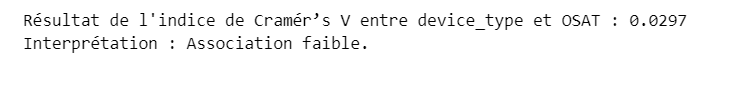
\includegraphics[width=0.6\linewidth]{capture_sas_38.png}
%     \caption{Résultat de l'indice de Cramér's V pour la variable \textbf{device\_type} et \textbf{OSAT}.}
%     \label{AnB1}
% \end{figure}

\begin{figure}[H]
    \centering
    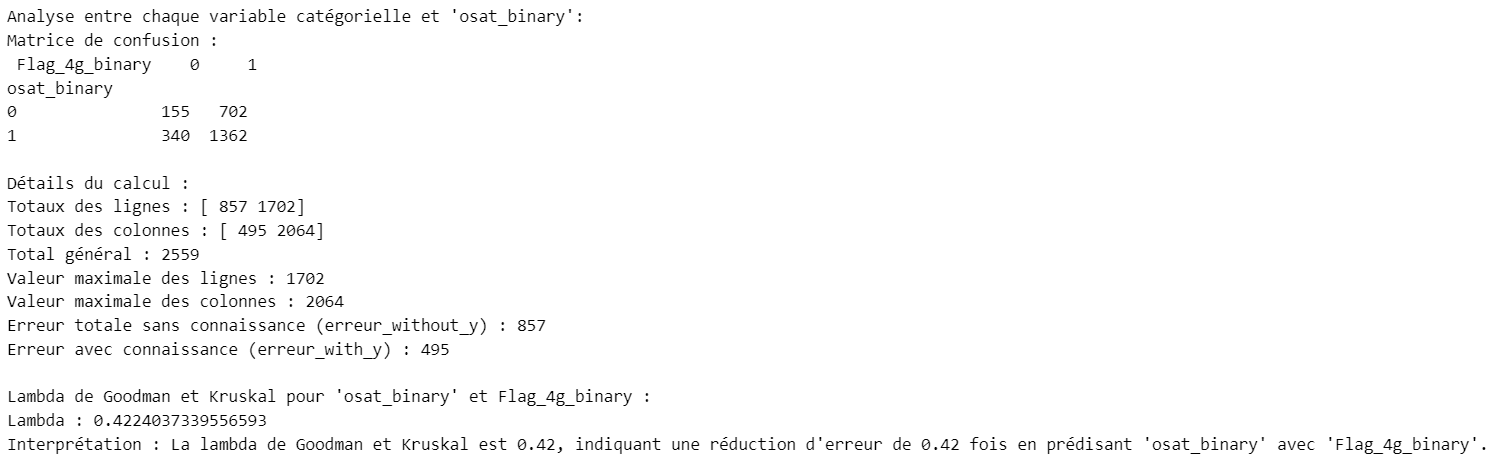
\includegraphics[width=0.9\linewidth]{capture_sas_40.png}
    \caption{Résultat de la Lambda de Goodman et Kruskal pour \textbf{Flag\_4g\_binary}.}
    \label{AnB2}
\end{figure}

\begin{figure}[H]
    \centering
    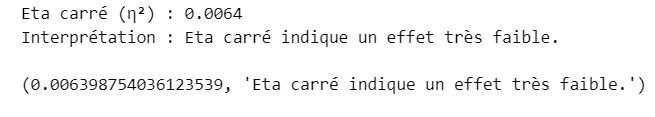
\includegraphics[width=0.8\linewidth]{capture_sas_41.png}
    \caption{Résultat de l'Eta carré pour \textbf{osat\_binary}}
    \label{AnB3}
\end{figure}

\begin{figure}[H]
    \centering
    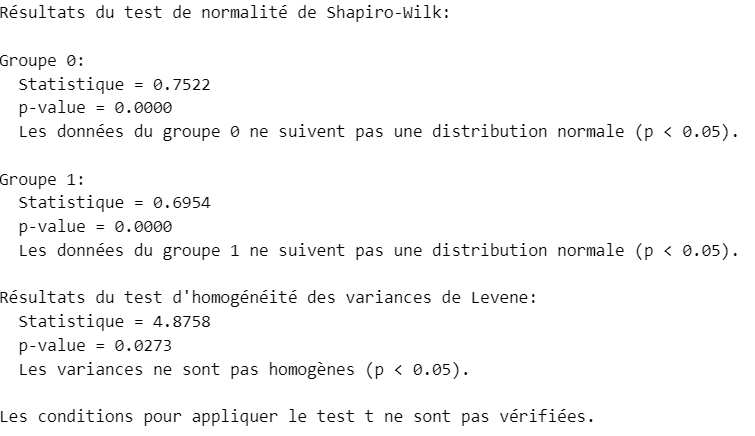
\includegraphics[width=0.8\linewidth]{capture_sas_42.png}
    \caption{Résultats du test de normalité et de variances}
    \label{AnB4}
\end{figure}

\begin{figure}[H]
    \centering
    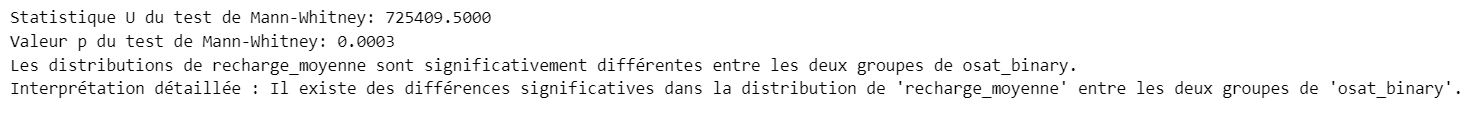
\includegraphics[width=0.8\linewidth]{capture_sas_43.png}
    \caption{Résultats du test de Mann-Whitney}
    \label{AnB5}
\end{figure}



\begin{figure}[H]
    \centering
    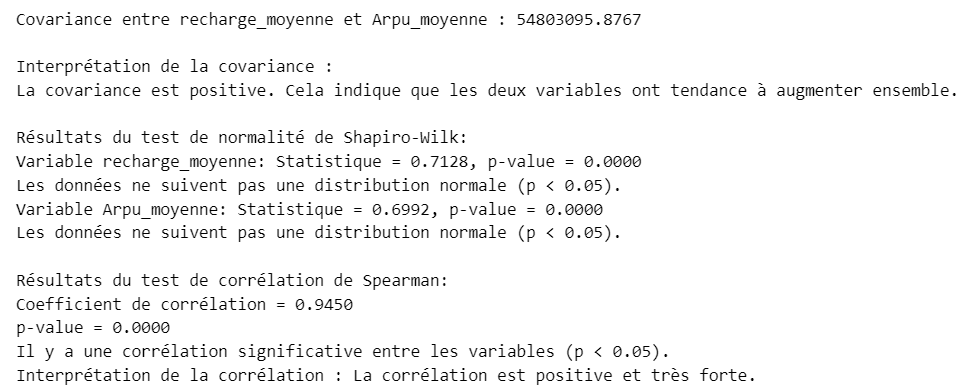
\includegraphics[width=0.8\linewidth]{capture_sas_49.png}
    \caption{Interprétation des résultats statistiques entre les deux variables}
    \label{11}
\end{figure}
